\subsection{Formal}
\label{sbsc:boundaries_formal}

Let's now turn to concrete definitions and bounds.
Remind that we are looking at the horizontal rectangle $\D$.

Suppose that $i_1 \equiv i_2 \pmod 2$, $i_1$ is even.
(If $i_1$ is odd, then $\D'$ and $\D''$ are swapped.)

\subsubsection{Bounds for $\D'$}

\begin{enumerate}[I.]
	\item Suppose both $\{\g_0(\M)\}$ and $\{\d_0(\M)\}$
	satisfy \ref{eq:cont-frac-left-normal} and the rectangle $\D$ is left-normal,
	that is, satisfies \ref{eq:left-normal}.
	We will denote such situation by $N-N-N$
	(segment $\D_1$ is left-normal, $\D_2$ is left-normal, rectangle $\D$ is normal).
	
	In this case define $\D'$ by equation
	\begin{equation}
		\D' = f(\overline{21}3a_{i_1}... a_{i_2}3\overline{12}).
	\end{equation}
	
	\item[IIa.] Sets $\{\g_0(\M)\}$ and $\{\d_0(\M)\}$
	meet condition \ref{eq:cont-frac-left-normal}
	and $\D$ is left-shortened, that is, meets condition \ref{eq:left-shortened}.
	This is case $N-N-S$
	(segments $\D_1$ and $\D_2$ are left-normal, rectangle $\D$ is left-shortened).
	
	Then
	\begin{equation}\label{eq:bound-l-nns}
		\D' = f(\overline{21}3a_{i_1}... a_{i_2}213\overline{12}).
	\end{equation}
	
	\item[IIb.] Set $\{\g_0(\M)\}$ meets \ref{eq:cont-frac-left-normal},
	$\{\d_0(\M)\}$ meets \ref{eq:cont-frac-left-shortened}.
	No matter which condition \ref{eq:left-shortened} of \ref{eq:left-normal} is met.
	It is the case $N-S$
	(segment $\D_1$ is left-normal, segment $\D_2$ left-shortened).
	Bound $\D_1$ is defined by \ref{eq:bound-l-nns}.
	
	\addtocounter{enumi}{1}
	\item Set $\{\g_0(\M)\}$ meets \ref{eq:cont-frac-left-shortened},
	$\{\d_0(\M)\}$ meets \ref{eq:cont-frac-left-normal}.
	In this $S-N$ case
	(segment $\D_1$ is left-shortened, segment $\D_2$ is left-normal)
	$\D'$ is defined as follows:
	\begin{equation}
		\D' = f(\overline{21}312a_{i_1}... a_{i_2}3\overline{12}).
	\end{equation}
	
	\item Both $\{\g_0(\M)\}$ and $\{\d_0(\M)\}$
	meet \ref{eq:cont-frac-left-shortened}.
	In this $S-S$ case
	(both segments $\D_1$ and $\D_2$ are left-shortened)
	$\D'$ is defined by
	\begin{equation}
		\D' = f(\overline{21}312a_{i_1}... a_{i_2}213\overline{12}).
	\end{equation}
\end{enumerate}

\begin{figure}[p]
	\centering
	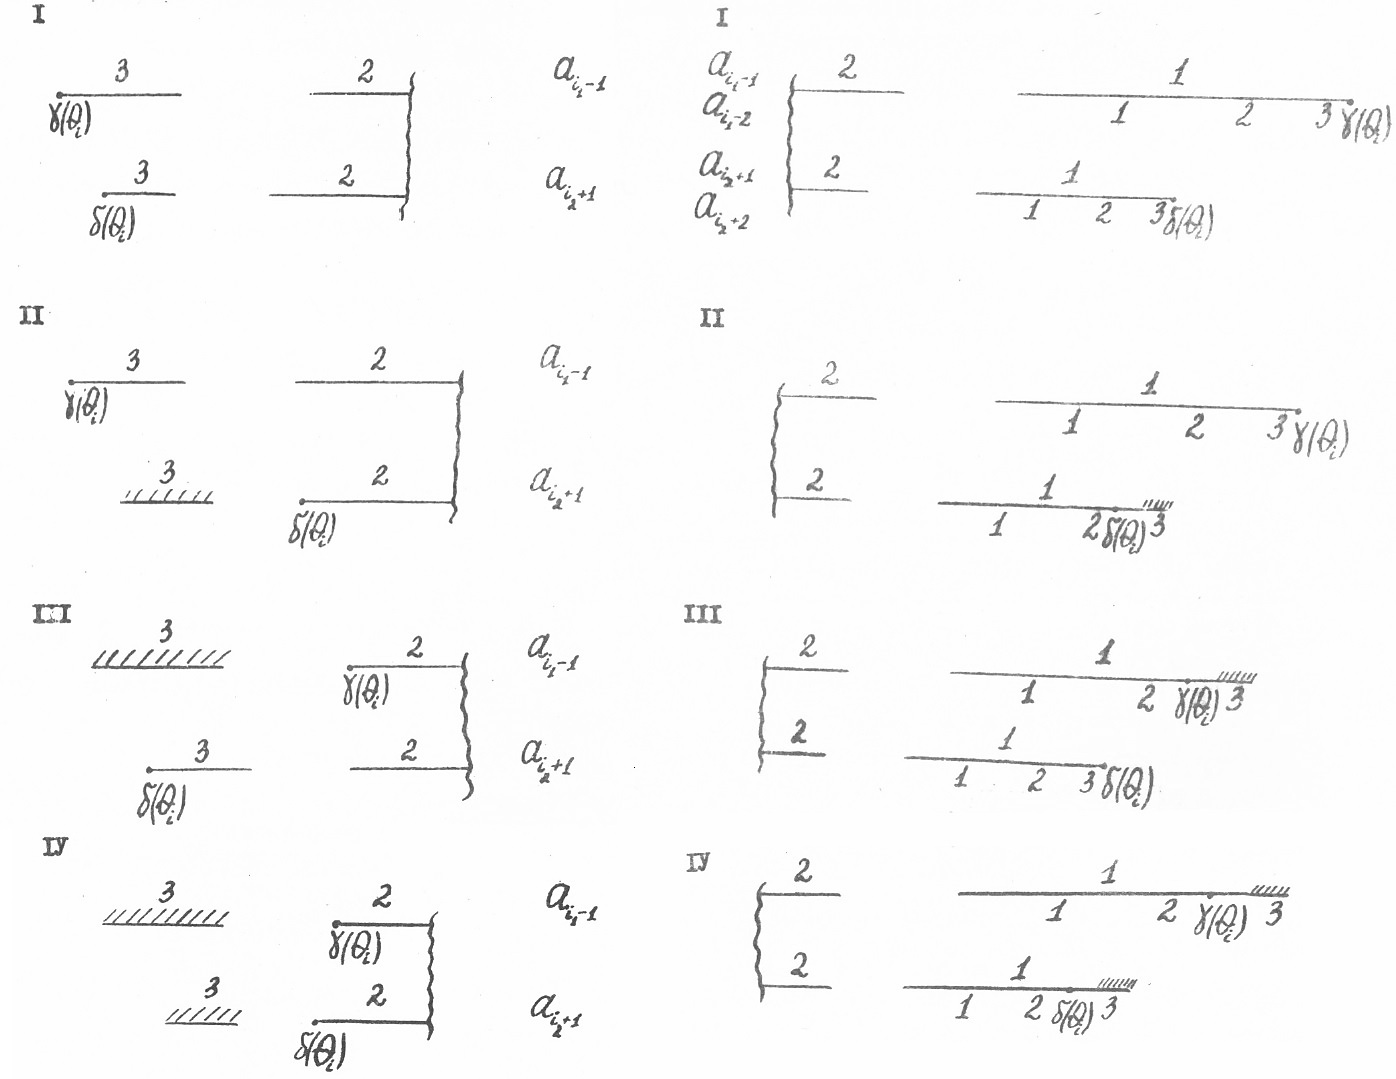
\includegraphics[width=0.9\textwidth]{rectangle-bounds-even}
	\caption{
		Bounds $\D'$ (left) and $\D''$ (right).\\
		Hatched areas correspond to values of $a_{i_1 - 1}$ and $a_{i_2 + 1}$ (on the left)
		or $a_{i_1 - 2}$ and $a_{i_2 + 2}$ (on the right), equal to 3,
		which can not appear in the concrete case. \\
		$\D_1' = \g(\T{i})$, $i=3,30$,
		$\D_2' = \d  (\T{i})$, $i=3,30$,
		$\D' = \D_1' + \D_2'$. \\
		$\D_1'' = \g(\T{i})$, $i = 90, 94$,
		$\D_2'' = \d  (\T{i})$, $i = 90, 94$.
	}
	\label{fg:rectangle-bounds-even}
\end{figure}

Left side of the figure \oldref{fg:rectangle-bounds-even} illustrates these bounds.

\subsubsection{Bounds for $\D''$}
Now we will provide formulas for $\D''$:

\begin{subequations}
	\begin{align}
		\label{eq:bound-r-nnn}
		&&&&& I & \D'' & = f(\overline{21}31a_{i_1}... a_{i_2}13\overline{12}), &&&& \\
		\label{eq:bound-r-nns-ns}
		&&&&& II & \D'' & = f(\overline{21}31a_{i_1}... a_{i_2}1213\overline{12}), &&&& \\
		\label{eq:bound-r-ns}
		&&&&& III & \D'' & = f(\overline{21}3121a_{i_1}... a_{i_2}13\overline{12}), &&&& \\
		\label{eq:bound-r-sn}
		&&&&& IV & \D'' & = f(\overline{21}3121a_{i_1}... a_{i_2}1213\overline{12}). &&&&
	\end{align}
\end{subequations}

Figure \ref{fg:rectangle-r-bound-choise} regulates the choise of the formulas.

\begin{figure}[ht]
	\centering
		\begin{tabular}{| l | c c c | c |}
			\cline{1-5}
				Case &
				$\D_1''$ &
				$\D_2''$ &
				Rectangle &
				$\D''$
			\\
			\cline{1-5}
				I &
				\ref{eq:cont-frac-right-normal} &
				\ref{eq:cont-frac-right-normal} &
				\ref{eq:right-normal} $N-N-N$ &
				\ref{eq:bound-r-nnn}
			\\
				IIa &
				\ref{eq:cont-frac-right-normal} &
				\ref{eq:cont-frac-right-normal} &
				\ref{eq:right-shortened} $N-N-S$ &
				\ref{eq:bound-r-nns-ns}
			\\
				IIb &
				\ref{eq:cont-frac-right-normal} &
				\ref{eq:cont-frac-right-shortened} &
				$N-S$ &
				\ref{eq:bound-r-nns-ns}
			\\
				III &
				\ref{eq:cont-frac-right-shortened} &
				\ref{eq:cont-frac-right-normal} &
				$S-N$ &
				\ref{eq:bound-r-ns}
			\\
				IV &
				\ref{eq:cont-frac-right-shortened} &
				\ref{eq:cont-frac-right-shortened} &
				$S-S$ &
				\ref{eq:bound-r-sn}
			\\
			\cline{1-5}
		\end{tabular}
	\caption{Rules for choise of $\D''$ in case $i_1 \equiv i_2 \pmod 2$.}
	\label{fg:rectangle-r-bound-choise}
\end{figure}

Again, these bounds are illustrated on the right side of the figure \oldref{fg:rectangle-bounds-even}.

\subsubsection{Case $i_1 \not\equiv i_2 \pmod 2$}

Now consider case $i_1 \not\equiv i_2 \pmod 2$, $i_1$ is even.
We will use rules from figure \ref{fg:rectangle-l-odd-bound-choise} to choose one of 4 formulas for $\D'$.

\begin{subequations}
	\begin{align}
		\label{eq:bound-l-odd-nn}
		&&&&& I & \D' & = f(\overline{21}3a_{i_1}... a_{i_2}13\overline{12}), &&&& \\
		\label{eq:bound-l-odd-ns}
		&&&&& II & \D' & = f(\overline{21}3a_{i_1}... a_{i_2}1213\overline{12}), &&&& \\
		\label{eq:bound-l-odd-sn}
		&&&&& III & \D' & = f(\overline{21}312a_{i_1}... a_{i_2}13\overline{12}), &&&& \\
		\label{eq:bound-l-odd-ss}
		&&&&& IV & \D' & = f(\overline{21}312a_{i_1}... a_{i_2}1213\overline{12}). &&&&
	\end{align}
\end{subequations}

\begin{figure}[ht]
	\centering
	\begin{tabular}{| l | c c c | c |}
		\cline{1-5}
		Case & $\D_1''$ & $\D_2''$ & Case name & $\D''$ \\
		\cline{1-5}
			I &
			\ref{eq:cont-frac-left-normal} &
			\ref{eq:cont-frac-right-normal} &
			$N-N$ &
			\ref{eq:bound-l-odd-nn}
		\\
			II &
			\ref{eq:cont-frac-left-normal} &
			\ref{eq:cont-frac-right-shortened} &
			$N-S$ &
			\ref{eq:bound-l-odd-ns}
		\\
			III &
			\ref{eq:cont-frac-left-shortened} &
			\ref{eq:cont-frac-right-normal} &
			$S-N$ &
			\ref{eq:bound-r-ns}
		\\
			IV &
			\ref{eq:cont-frac-left-shortened} &
			\ref{eq:cont-frac-right-shortened} &
			$S-S$ &
			\ref{eq:bound-r-sn}
		\\
		\cline{1-5}
	\end{tabular}
	\caption{Rules for choise of $\D'$ in case $i_1 \not\equiv i_2 \pmod 2$, $i_1$ is even.}
	\label{fg:rectangle-l-odd-bound-choise}
\end{figure}

To determine the bound $\D''$, we will use subrectangle
\begin{equation*}
	\{1, 0\}.
\end{equation*}
Having $i_1 - 1 \equiv i_2 \pmod 2$, so we can use all the previous formulas to determine $\D''$.
